\begin{problem}[1]
  Evaluate the following double integrals over the given regions.
  \begin{enumerate}
    \item $\displaystyle \iint_R ye^{xy} \,\dA$ where $R = [0, 2] \times [0,
      4]$.

    \item $\displaystyle \iint_D y\sqrt{x^2 - y^2} \,\dA$ where $D$ is the
      triangle with vertices $(0, 0)$, $(2, 0)$, and $(2, 2)$.

    \item $\displaystyle \iint_D 2xy^3 \,\dA$ where $D$ is the region bounded by $y = x$, $y = \frac{1}{x}$, and $y = 2$.
  \end{enumerate}
\end{problem}

\begin{proof}[Solution to (i)]
  Graphing the bounds gives us the following figure.
  \begin{center}
    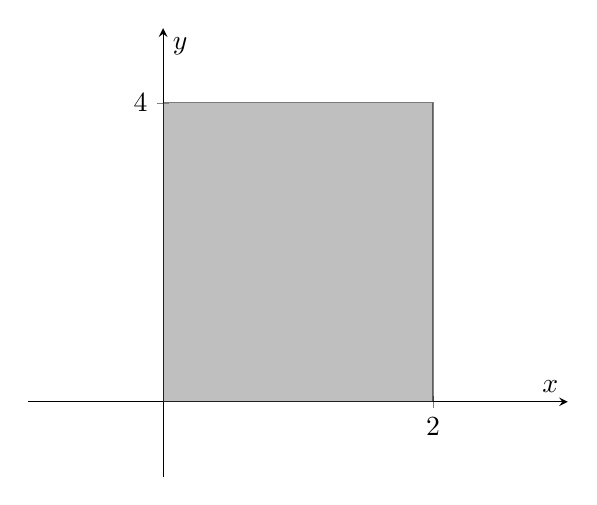
\begin{tikzpicture}
      \begin{axis}[
        axis lines = center,
        xlabel = $x$,
        ylabel = $y$,
        xmin = -1, xmax = 3,
        ymin = -1, ymax = 5,
        xtick = {0, 2},
        ytick = {0, 4},
        xticklabels = {$0$, $2$},
        yticklabels = {$0$, $4$},
      ]
        \addplot[fill=gray, opacity=0.5] coordinates {
            (0,0) (0,4) (2,4) (2,0) (0,0)
        };
      \end{axis}
    \end{tikzpicture}
  \end{center}
  Therefore, we get the bounds $0 \le x \le 2$ and $0 \le y \le 4$. Expanding
  the double integral into an iterated integral and evaluating gives us
  \begin{align*}
    \iint_R ye^{xy} \,\dA &= \int_0^4 \int_0^2 ye^{xy} \,\dx \,\dy \\
                          &= \int_0^4 \left[e^{xy}\right]_0^2 \,\dy \\
                          &= \int_0^4 e^{2y} - 1 \,\dy \\
                          &= \left[\frac{e^{2y}}{2} - y\right]_0^4 \\
                          &= \frac{1}{2}(e^8 - 9)
  .\qedhere\end{align*}
\end{proof}

\begin{proof}[Solution to (ii)]
  Graphing the bounds gives us the following figure.
  \begin{center}
    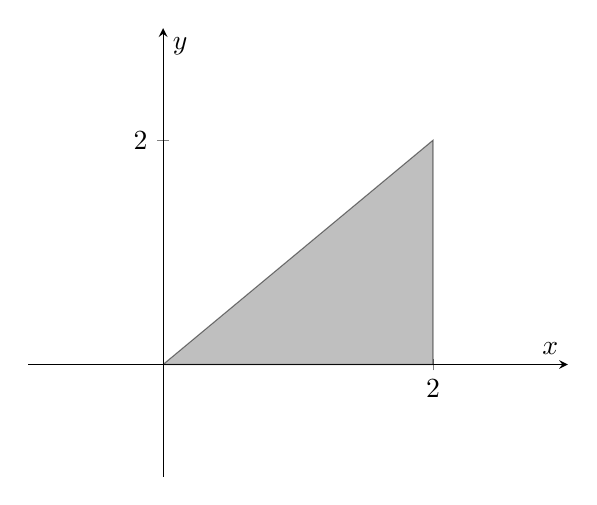
\begin{tikzpicture}
      \begin{axis}[
        axis lines = center,
        xlabel = $x$,
        ylabel = $y$,
        xmin = -1, xmax = 3,
        ymin = -1, ymax = 3,
        xtick = {0, 2},
        ytick = {0, 2},
        xticklabels = {$0$, $2$},
        yticklabels = {$0$, $2$},
      ]
        \addplot[fill=gray, opacity=0.5] coordinates {
          (0, 0) (2, 0) (2, 2) (0, 0)
        };
      \end{axis}
    \end{tikzpicture}
  \end{center}
  Therefore, we get the bounds $0 \le x \le 2$ and $0 \le y \le x$. Expanding
  the double integral into an iterated integral gives us
  \[%
    \iint_D y\sqrt{x^2 - y^2} \,\dA = \int_0^2 \int_0^x y\sqrt{x^2 - y^2} \,\dy \,\dx
  .\]%
  Using a $u$-substitution of $u = y^2$, we have $\du = 2y\,\dy$. The bounds go
  from $0 \mapsto 0$ and $x \mapsto x^2$. This simplifies the integral to
  \begin{align*}
    \int_0^2 \int_0^x y\sqrt{x^2 - y^2} \,\dy \,\dx &= \int_0^2 \int_0^{x^2} \frac{1}{2} \sqrt{x^2 - u} \,\du \,\dx \\
                                                    &= \int_0^2 \int_0^{x^2} \frac{1}{2} (x^2 - u)^{\sfrac{1}{2}} \,\du \,\dx \\
                                                    &= \int_0^2 \frac{1}{2} \left[-\frac{(x^2 - u)^{\sfrac{3}{2}}}{\sfrac{3}{2}}\right]_0^{x^2} \,\dx \\
                                                    &= \int_0^2 \frac{1}{\rcancel{2}} \cdot \frac{\rcancel{2}}{3} \left[-\frac{(x^2 - u)^{\sfrac{3}{2}}}{\sfrac{3}{2}}\right]_0^{x^2} \,\dx \\
                                                    &= \int_0^2 -\frac{1}{3} \left[(x^2 - 0)^{\sfrac{3}{2}}\right] - \left[(x^2 - 0)^{\sfrac{3}{2}}\right] \,\dx \\
                                                    &= \int_0^2 \frac{1}{3} \left(x^2\right)^{\sfrac{3}{2}} \,\dx \\
                                                    &= \int_0^2 \frac{1}{3} x^3 \,\dx \\
                                                    &= \frac{1}{3} \cdot \left. \frac{x^4}{4} \right\rvert_0^2 \\
                                                    &= \frac{1}{3} \cdot \left[\frac{2^4}{4} - \frac{0^4}{4}\right] \\
                                                    &= \frac{1}{3} \cdot \frac{16}{4} \\
                                                    &= \frac{4}{3}
  .\qedhere\end{align*}
\end{proof}

\begin{proof}[Solution to (iii)]
  Graphing the bounds gives us the following figure.
  \begin{center}
    \begin{tikzpicture}
      \begin{axis}[
        axis lines = center,
        xlabel = $x$,
        ylabel = $y$,
        xmin = 0.4, xmax = 2.4,
        ymin = 0.6, ymax = 2.4,
        ]
        \addplot[domain=1:2] {x} node[midway, right] {$y = x$};
        \addplot[domain=0.5:1] {1/x} node[midway, right] {$y = \frac{1}{x}$};
        \addplot[domain=0.5:2] {2} node[midway, below] {$y = 2$};
      \end{axis}
    \end{tikzpicture}
  \end{center}
  Therefore, we get the bounds $1 \le y \le 2$ and $y \le x \le \frac{1}{y}$.
  Expanding the double integral into an iterated integral and evaluating gives
  us
  \begin{align*}
    \iint_D 2xy^3 \,\dA &= \int_1^2 \int_{\sfrac{1}{y}}^y 2xy^3 \,\dx \,\dy \\
                        &= \int_1^2 y^2 y_3 - \frac{y^3}{y^2} \,\dy \\
                        &= \int_1^2 y^5 - y \,\dy \\
                        &= \left. \frac{y^6}{6} - \frac{y^2}{2} \right\rvert_1^2 \\
                        &= \frac{2^6}{6} - 2 - \frac{1}{6} + \frac{1}{2} \\
                        &= 9
  .\qedhere\end{align*}
\end{proof}

\begin{problem}[2]
  By changing the order of integration, evaluate the integral
  \[%
    \int_0^2 \int_{x^2}^4 \sqrt{y} \sin(y) \,\dy \,\dx
  .\]%
\end{problem}

\begin{proof}[Solution]
  Graphing the bounds gives us the following figure.
  \begin{center}
    \begin{tikzpicture}
      \begin{axis}[
        xmin = -1, xmax = 3,
        ymin = -1, ymax = 5,
        xtick = {0, 2},
        ytick = {0, 4},
        xticklabels = {$0$, $2$},
        yticklabels = {$0$, $4$},
      ]
        \addplot[-, samples=1000, domain=0:2] {x^2} node[midway, right] {$y = x^2$};
        \addplot[-, domain=0:2] {4} node[midway, below] {$y = 4$};
      \end{axis}
    \end{tikzpicture}
  \end{center}
  Solving the equation $y = x^2$ gives us $x = \pm\sqrt{y}$. But we only want
  the positive root. Therefore, we get the bounds $0
  \le y \le 4$ and $0 \le x \le \sqrt{y}$. Expanding the double integral into an iterated integral gives us
  \begin{align*}
    \iint_R \sqrt{y} \sin(y) \,\dA &= \int_0^4 \int_0^{\sqrt{y}} \sqrt{y} \sin(y) \,\dx \,\dy \\
                                   &= \int_0^4 \sqrt{y} \sin(y) \cdot x \rvert_0^{\sqrt{y}} \,\dy \\
                                   &= \int_0^4 y \sin(y) \,\dy
  .\end{align*}
  Using integration by parts gives us
  \begin{align*}
    \begin{rcases}
      &\phantom{d}u = y \quad \dv = \sin(y) \,\dy \\
      &\du = \dy \quad v = -\cos(y)
    \end{rcases} \implies \int_0^4 y \sin(y) \,\dy &= \left[-y \cos(y) - \int -\cos(y) \,\dy\right]_0^4 \\
                                                   &= \left[\sin(y) - 4\cos(y)\right]_0^4 \\
                                                   &= 4\sin(4) - 4\cos(4)
  .\qedhere\end{align*}
\end{proof}

\begin{problem}[3]
  Use a double integral to find the volume of the following solids.
  \begin{enumerate}
    \item The solid that is bounded by the coordinate planes and the plane $2x +
      3y + z = 6$.

      Note: This solid is a tetrahedron. It can be easily drawn by using the
      lines of intersection between the slant plane and the coordinate planes.

   \item The solid enclosed by the parabolic cylinder $y = 2 - x^2$ and the
     planes $z = 2 - y$, $y = x$, and $z = 0$

      Note : Surfaces that do not depend on $z$ are vertical surfaces.
  \end{enumerate}
\end{problem}

\begin{proof}[Solution to (i)]
  The points of intersection are
  \begin{alignat*}{5}
    &\textrm{At}~x = 0 = y &&\implies z = 6 \\
    &\textrm{At}~y = 0 = z &&\implies x = 3 \\
    &\textrm{At}~z = 0 = x &&\implies y = 2
  .\end{alignat*}
  The projection of the plane onto the $xy$-plane forms a triangle with vertices
  $(0, 0)$, $(3, 0)$, and $(0, 2)$. Solving for the equation of the line gives
  us
  \[%
    y = -\frac{2}{3}x + 2
  .\]%
  Graphing the bounds gives us the following figure.
  \begin{center}
    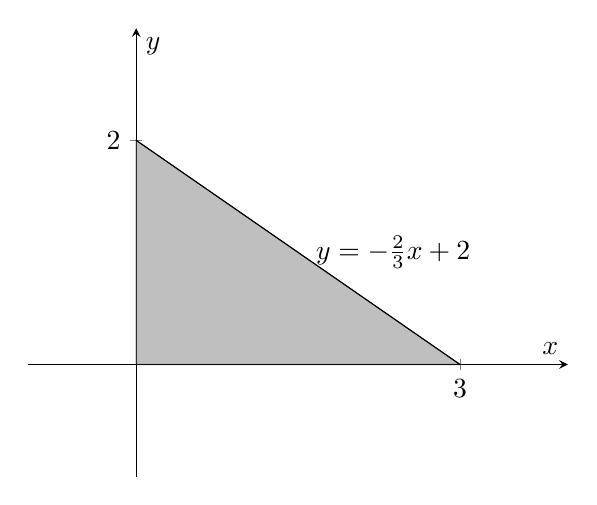
\begin{tikzpicture}
      \begin{axis}[
        axis lines = center,
        xlabel = $x$,
        ylabel = $y$,
        xmin = -1, xmax = 4,
        ymin = -1, ymax = 3,
        xtick = {0, 3},
        ytick = {0, 2},
        xticklabels = {$0$, $3$},
        yticklabels = {$0$, $2$},
      ]
        \addplot[fill=gray, opacity=0.5] coordinates {
          (0, 0) (3, 0) (0, 2) (0, 0)
        };
        \addplot[domain=0:3] {-2/3*x + 2} node[midway, right, xshift=0.3em] {$y = -\frac{2}{3}x + 2$};
      \end{axis}
    \end{tikzpicture}
  \end{center}
  The equation of the plane can be written as $f(x, y) = 6 - 2x - 3y$.
  Therefore, we get the bounds for $x$ to be $0 \le x \le 3$ and the bounds for
  $y$ to be $0 \le y \le -\frac{2}{3}x + 2$. The volume is then and evaluating
  using Wolfram Alpha to get
  \begin{align*}
    V = \int_0^3 \int_0^{-\frac{2}{3}x + 2} 6 - 2x - 3y \,\dy \,\dx &= \int_0^3 6\left[-\frac{2}{3}x + 2\right] - 2\left[-\frac{2}{3}x + 2\right] - \frac{3}{2} \left[-\frac{2}{3} + 2\right]^2 \,\dy \,\dx \\
                                                                    &= \int_0^3 12 - 4x - 4x + \frac{4x^2}{3} - \frac{3}{2}\left[4 - \frac{4}{3}x - \frac{4}{3}x + \frac{4}{9}x^2\right] \,\dx \\
                                                                    &= \int_0^3 12 - 4x - 4x + \frac{4x^2}{3} - 6 + 2x + 2x - \frac{72x^2}{78} \,\dx \\
                                                                    &= \int_0^3 6 - 4x + \frac{2x^2}{3} \,\dx \\
                                                                    &= \left. 6x - \frac{4x^2}{2} + \frac{2x^3}{9} \right\rvert_0^3 = 18 - 18 + 6 = 6
  .\qedhere\end{align*}
\end{proof}

\begin{proof}[Solution to (ii)]
  Since $x = y = 2 - x^2$, we get $x^2 + x - 2 = 0$. Solving for $x$ gives us $x
  = -2$ and $x = 1$. Therefore, the bounds for $x$ are $-2 \le x \le 1$. The
  bounds for $y$ are $x \le y \le 2 - x^2$. Graphing the bounds gives us the
  following figure.
  \begin{center}
    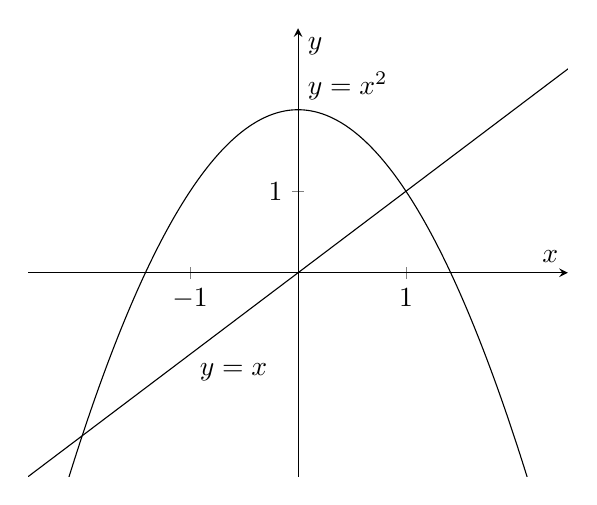
\begin{tikzpicture}
      \begin{axis}[
        axis lines = center,
        xlabel = $x$,
        ylabel = $y$,
        xmin = -2.5, xmax = 2.5,
        ymin = -2.5, ymax = 3,
        xtick = {-1, 1},
        ytick = {1},
        xticklabels = {$-1$, $1$},
        yticklabels = {$1$},
      ]
        \addplot[samples=1000, domain=-3:3] {2 - x^2};
        \addplot[samples=1000] {x};

        \draw (0, 2) node[above right] {$y = x^2$};
        \draw (-1, -1) node[below right] {$y = x$};
      \end{axis}
    \end{tikzpicture}
  \end{center}
  Therefore, expanding the double integral into an iterated integral gives us
  \begin{align*}
    V = \int_{-2}^1 \int_x^{2 - x^2} 2 - y \,\dy \,\dx &= \int_{-2}^1 \left. 2y - \frac{y^2}{2} \right\rvert_x^{2 - x^2} \,\dx \\
                                                       &= \int_{-2}^1 \left[2(2 - x^2) - \frac{(2 - x^2)^2}{2}\right] - \left[2x - \frac{x^2}{2}\right] \,\dx \\
                                                       &= \int_{-2}^1 \left[4 - 2x^2 - \frac{4 - 4x^2 + x^4}{2}\right] - \left[2x - \frac{x^2}{2}\right] \,\dx \\
                                                       &= \int_{-2}^1 4 - 2x^2 - 2 + 2x^2 - \frac{x^4}{2} - 2x + \frac{x^2}{2} \,\dx \\
                                                       &= \int_{-2}^1 2 - 2x + \frac{x^2}{2} - \frac{x^4}{2} \,\dx \\
                                                       &= \left. 2x - x^2 + \frac{x^3}{6} - \frac{x^5}{10} \right\rvert_{-2}^1 \\
                                                       &= \left[2 - 1 + \frac{1}{6} - \frac{1}{10}\right] - \left[-4 - 4 - \frac{8}{6} + \frac{32}{10}\right] \\
                                                       &= \frac{36}{5}
  .\qedhere\end{align*}
\end{proof}
